\documentclass[11pt]{article}
\usepackage{fullpage}
\usepackage{fancyhdr}
\usepackage{epsfig}
\usepackage{algorithm}
\usepackage[noend]{algorithmic}
\usepackage{amsmath,amssymb,amsthm}
\usepackage{graphicx}



% FILL IN THE SPECIFICS OF EACH HOMEWORK HERE
\newcommand{\course}{Music 421a}
\newcommand{\semester}{Winter 2012}
\newcommand{\name}{Audio Applications of the FFT}
\newcommand{\hwk}{Homework \#5 Solutions}
\newcommand{\student}{Hunter McCurry}


%%
% The following are definitions so that you can use numbered lemmas, claims, etc.
%%
\newtheorem{lemma}{Lemma}
\newtheorem*{lem}{Lemma}
\newtheorem{definition}{Definition}
\newtheorem{notation}{Notation}
\newtheorem*{claim}{Claim}
\newtheorem*{fclaim}{False Claim}
\newtheorem{observation}{Observation}
\newtheorem{conjecture}[lemma]{Conjecture}
\newtheorem{theorem}[lemma]{Theorem}
\newtheorem{corollary}[lemma]{Corollary}
\newtheorem{proposition}[lemma]{Proposition}

%%
% The following are definitions so that you can use some shorthand with deltas and such
%%
\newcommand{\deltahat}{\hat{\delta}}
\newcommand{\Deltahat}{\hat{\Delta}}
\newcommand{\righti}{\stackrel{i}{\rightarrow}}
\newcommand{\rights}{\stackrel{*}{\rightarrow}}
\newcommand{\righto}{\stackrel{1}{\rightarrow}}
\newcommand{\rightn}{\stackrel{n}{\rightarrow}}
\newcommand{\rightnp}{\stackrel{n+1}{\rightarrow}}
\newcommand{\rightip}{\stackrel{i+1}{\rightarrow}}
\newcommand{\rightk}{\stackrel{k}{\rightarrow}}
\newcommand{\rightln}{\stackrel{\leq n}{\rightarrow}}



%%% You can ignore the following stuff, it's just for formatting purposes
\textheight=8.6in
\setlength{\textwidth}{6.44in}
\addtolength{\headheight}{\baselineskip} 
% enumerate uses a), b), c), ...
\renewcommand{\labelenumi}{\alph{enumi})}
% Sets the style for fancy pages (namely, all but first page)
\pagestyle{fancy}
\fancyhf{}
\renewcommand{\headrulewidth}{0.0pt}
\renewcommand{\footrulewidth}{0.4pt}
% Changes style of plain pages (namely, the first page)
\fancypagestyle{plain}{
  \fancyhf{}
  \renewcommand\headrulewidth{0pt}
  \renewcommand\footrulewidth{0.4pt}
  \renewcommand{\headrule}{}
  }
% Changes the title box on the first page
\renewcommand\maketitle{
\begin{center}
\begin{tabular*}{6.44in}{l @{\extracolsep{\fill}}c r}
\bfseries  &  & \bfseries \course ~\semester \\
\bfseries&  & \bfseries  \hwk  \\
\bfseries   &   &  \bfseries \student \\ 
\end{tabular*}
\end{center} }




%%
%%
%% THE REAL STUFF STARTS HERE
%%
%%
\begin{document}
\maketitle
\thispagestyle{plain}


\noindent 


\subsection*{Question 1}
\begin{enumerate}
\item For a rectangular window of length 255, we will end up with 255 frequency bins (including 0 Hz) after we take the transform. Given that our sampling rate is 8192 Hz, and that our frequency bins will be equally spaced, our bins will occur every 32.125 Hz. This means that our closest bin to 440 Hz will fall at 449.757 Hz.

\begin{eqnarray*}
\Delta f = |f_0 - \hat f | / f_0 =  |449.757 - 440| / 440 =  0.022 \\
\end{eqnarray*}

\item Instead of 255 frequency bins, we will now have 1275 bins, meaning our bins will occur every 6.425 Hz. The closest bin will fall at 436.906 Hz.

\begin{eqnarray*}
\Delta f = |f_0 - \hat f | / f_0 =  |436.906 - 440| / 440 =  0.007 \\
\end{eqnarray*}

\item 

\begin{verbatim}
% Problem 1c matlab code
f = 440;
M = 255;
fs = 8192;
rect = ones(1, M);
sinusoid = .6 * cos( ((f * 2 * pi) / fs) * (0:(M-1)) );
sin_padded = zeropadzerophasewin(sinusoid, rect, 5 * M);
sinTr = fft( sin_padded );
stem([0:fs/(5*M):fs*(1-1/(5*M))]-(fs/2), ...
abs(fftshift(sinTr))/max(abs(fftshift(sinTr))));
\end{verbatim}

\begin{figure}[!h]
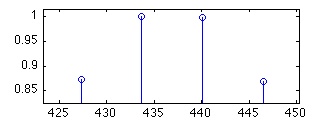
\includegraphics[scale=.75]{1a_peak}
\end{figure}

Note that the graph is plotted in linear amplitude. As the amplitude levels are close to even on each side of the peak we can guess make a guess at the peak by averaging the two highest levels (433.69 Hz and 440.12 Hz) to get 436.91 Hz.

\begin{eqnarray*}
\Delta f = |f_0 - \hat f | / f_0 =  |436.91 - 440| / 440 =  0.007 \\
\end{eqnarray*}

\end{enumerate}


\subsection*{Question 2}
\begin{enumerate}
\item By following the same steps taken in the section of the book entitled 'Sinusoidal Amplitude and Phase Estimation', we can find the amplitude and phase that best estimates our sinusoid, even if an additional sinusoid $s(n)$ is added into it. Essentially, all combinations of our two variables $A$ and $\phi$ form a plane. There will be a single closest point on this plane to our signal $x(n)$	, and the coordinates $(A, \phi)$ of this point should be our answer. Following the steps taken in the book we end up with equation (6.42):

\begin{eqnarray*}
\mathcal{\hat A} = \hat A e ^ {j \hat \phi } = \frac{1}{N} \hbox{DTFT}_{\omega_{0}} (x) \\
\end{eqnarray*}

\item Since we know that there is a second sinusoid $s(n)$ contained within $x(n)$, we accept that it has the potential to add error to our estimate of $\mathcal{\hat A}$. First of all, if the frequency of $s(n)$ is the same or close to the known frequency $\omega_{0}$ of our target sinusoid, it may be impossible to separate the amplitudes and phases of the two sinusoids. More generally, no matter how far about the two sinusoids are in frequency, if the center of a side-lobe of $s(n)$ happens to correspond to $\omega_{0}$, it will add in error to our estimate. The only way to be sure that we will not have bias in $\mathcal{\hat A}$ is if $\omega_{0}$ falls on a null in the transform of $s(n)$.
\end{enumerate}


\subsection*{Question 3}

\begin{claim}
If e(n) denotes a sample of white noise, then the signal $x(n) = \textsc{Stretch}_{2}(e)$ is \emph{not} white noise.
\end{claim}

\begin{proof} (By Contradiction)
Let's say that we agree that $x(n)$ is white noise. Now we can apply the process again to obtain a new signal $y(n) = \textsc{Stretch}_{2}(x)$. Since $x(n)$ started out as white noise, and we agreed that \textsc{Stretch}ing by 2 produces more white noise, $y(n)$ is also white noise. We can continue this process indefinitely until we finally end up with a signal $z(n)$ which consists of an impulse followed by some (very large) number of zeros, followed by another impulse, followed by the same (very large) number of zeros, etc. By the stationary test, signal $z(n)$ fails to pass as white noise for the same reason that an impulse is not white noise. Namely, its statistics are not the same for every time instant. Since $z(n)$ doesn't pass as white noise, we have to assume that our process broke the instant we decided that $x(n)$ qualified as white noise.

\end{proof}

\subsection*{Question 4}
\begin{enumerate}
\item $[1, 0, 0, 0, 0, 0, 0, 0]$
\item $[2, 1, 0, 0, 0, 0, 0, 1]$
\item $[4, 3, 2, 1, 0, 1, 2, 3]$
\item $[8, 8, 8, 8, 8, 8, 8, 8]$
\end{enumerate}

\subsection*{Question 5}
\begin{enumerate}
\item $[1, 4, 10, 20, 31, 40, 44, 40, 31, 20, 10, 4, 1]$
\item Power Spectral Density is defined as the Fourier transform of the sample autocorrelation function (7.11 in the book). Starting from the autocorrelation obtained in part a), we take magnitude of the FFT:

$[ 256.00,  139.86,   16.39,    0.02,    0.42,    1.27,   0.05,    0.05,    1.27,    0.42,    0.02,   16.39,   139.86]$

\end{enumerate}


\end{document}
